\documentclass[aspectratio=169]{beamer}
\usetheme{Madrid}
\usecolortheme{seahorse}
\usepackage{amsmath}
\usepackage{amssymb}
\usepackage{tikz}
\usepackage{pgfplots}
\pgfplotsset{compat=1.16}
\usetikzlibrary{shapes.geometric, arrows.meta, positioning, calc}
\usepackage{pifont}           % Provides the dingbat symbols like \ding{55}
\usepackage{newunicodechar}   % Allows you to define Unicode characters
\newunicodechar{✓}{\checkmark}
\newunicodechar{✗}{\ding{55}}
% Colors
\definecolor{highDcolor}{RGB}{46, 134, 171}
\definecolor{lowDcolor}{RGB}{162, 59, 114}

\title{t-Stochastic Neighbor Embedding}
\subtitle{A Mathematical Journey}
\author{Advanced Multivariate Analysis}
\institute{UPC Barcelona}
\date{October 2025}

\begin{document}

% SLIDE 1
\begin{frame}
\titlepage
\end{frame}

% SLIDE 2
\begin{frame}
\frametitle{The Fundamental Problem}
\begin{columns}[T]
\column{0.5\textwidth}
\textbf{Given:}
\begin{itemize}
\item $\mathbf{X} = \{\mathbf{x}_1, \ldots, \mathbf{x}_n\}$
\item $\mathbf{x}_i \in \mathbb{R}^d$, $d \gg 2$
\end{itemize}
\textbf{Find:}
\begin{itemize}
\item $\mathbf{Y} = \{\mathbf{y}_1, \ldots, \mathbf{y}_n\}$
\item $\mathbf{y}_i \in \mathbb{R}^2$
\end{itemize}
\vspace{0.3cm}
\textbf{Information Loss:}
$$\text{Loss} = \frac{d - 2}{d} \times 100\%$$
$d = 100 \Rightarrow$ 98\% loss!

\column{0.5\textwidth}
\begin{center}
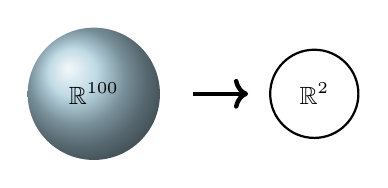
\begin{tikzpicture}[scale=0.7]
\shade[ball color=highDcolor!40] (0,0) circle (1.2cm);
\node at (0,0) {\small $\mathbb{R}^{100}$};
\draw[->, ultra thick] (1.8,0) -- (2.8,0);
\draw[thick] (4,0) circle (0.8cm);
\node at (4,0) {\small $\mathbb{R}^{2}$};
\end{tikzpicture}
\end{center}
\vspace{0.5cm}
\textbf{Key Question:}\\
Which 2\% of structure should we preserve?
\end{columns}
\end{frame}

% SLIDE 3
\begin{frame}
\frametitle{Distance Matrices}
\begin{columns}[T]
\column{0.5\textwidth}
\textbf{Distance Matrix:}
$$D_{ij} = \|\mathbf{x}_i - \mathbf{x}_j\|_2$$

Properties:
\begin{itemize}
\item Symmetric: $D_{ij} = D_{ji}$
\item Non-negative: $D_{ij} \geq 0$
\item Zero diagonal: $D_{ii} = 0$
\end{itemize}

\textbf{Can we embed exactly in $\mathbb{R}^2$?}\\
Usually NO!

\column{0.5\textwidth}
\textbf{Example: 4 points}
\begin{center}
\small
\begin{tabular}{c|cccc}
  & A & B & C & D \\
\hline
A & 0 & 1 & 1 & 1 \\
B & 1 & 0 & 1 & 1 \\
C & 1 & 1 & 0 & 1 \\
D & 1 & 1 & 1 & 0 \\
\end{tabular}
\end{center}
This is a tetrahedron!
\begin{itemize}
\item Needs $\mathbb{R}^3$ minimum
\item Cannot draw in $\mathbb{R}^2$
\end{itemize}
\end{columns}
\end{frame}

% SLIDE 4
\begin{frame}
\frametitle{The Curse of Dimensionality}
\begin{columns}[T]
\column{0.5\textwidth}
\textbf{Volume of $d$-sphere:}
$$V_d(r) \propto r^d$$

\textbf{Shell volume ratio:}\\
Inner radius = 0.9, Outer = 1.0
\begin{center}
\begin{tabular}{c|c}
Dim & In shell \\
\hline
2 & 19\% \\
10 & 65\% \\
100 & 99.997\% \\
\end{tabular}
\end{center}

\column{0.5\textwidth}
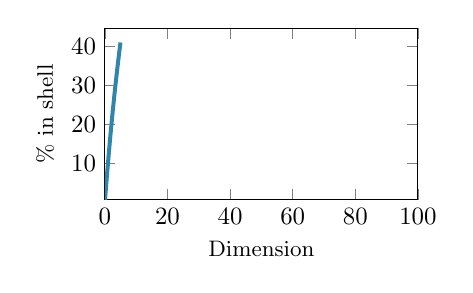
\begin{tikzpicture}[scale=0.9]
\begin{axis}[
    xlabel={\small Dimension},
    ylabel={\small \% in shell},
    width=6cm, height=4cm,
    xmin=0, xmax=100
]
\addplot[highDcolor, ultra thick] 
    {100*(1 - 0.9^x)};
\end{axis}
\end{tikzpicture}

\textbf{In high-D:} All points on boundary!
\end{columns}
\end{frame}

% SLIDE 5
\begin{frame}
\frametitle{The Crowding Problem}
\begin{columns}[T]
\column{0.45\textwidth}
\textbf{1000 points in $\mathbb{R}^{10}$}
\begin{itemize}
\item 99\% in shell $r \in [0.8, 1.0]$
\item Average distance $\approx 1.13$
\end{itemize}

\textbf{Project to $\mathbb{R}^2$:}
\begin{itemize}
\item Area ratio: $(0.8)^2 = 0.64$
\item 99\% must fit in 36\% area
\item \textcolor{red}{Crowding!}
\end{itemize}

\column{0.55\textwidth}
\begin{center}
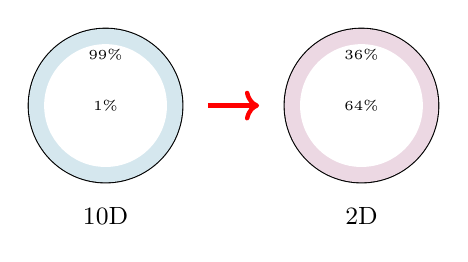
\begin{tikzpicture}[scale=0.65]
% 10D
\draw[thick] (0,0) circle (1.5cm);
\draw[thick] (0,0) circle (1.2cm);
\fill[highDcolor!20] (0,0) circle (1.5cm);
\fill[white] (0,0) circle (1.2cm);
\node at (0,0) {\tiny 1\%};
\node at (0,1) {\tiny 99\%};
\node[below] at (0,-1.8) {\small 10D};

\draw[->, ultra thick, red] (2,0) -- (3,0);

% 2D
\begin{scope}[shift={(5,0)}]
\draw[thick] (0,0) circle (1.5cm);
\draw[thick] (0,0) circle (1.2cm);
\fill[lowDcolor!20] (0,0) circle (1.5cm);
\fill[white] (0,0) circle (1.2cm);
\node at (0,0) {\tiny 64\%};
\node at (0,1) {\tiny 36\%};
\node[below] at (0,-1.8) {\small 2D};
\end{scope}
\end{tikzpicture}
\end{center}
\end{columns}
\end{frame}

% SLIDE 6
\begin{frame}
\frametitle{From Distances to Probabilities}
\begin{columns}[T]
\column{0.45\textwidth}
\textbf{Why Probabilities?}
\begin{itemize}
\item Distances: absolute
\item Probabilities: relative
\item Focus on local structure
\end{itemize}

\textbf{Transform:}
$$s_{ij} = \exp\left(-\frac{d_{ij}^2}{2\sigma_i^2}\right)$$
$$p_{j|i} = \frac{s_{ij}}{\sum_{k \neq i} s_{ik}}$$

\column{0.55\textwidth}
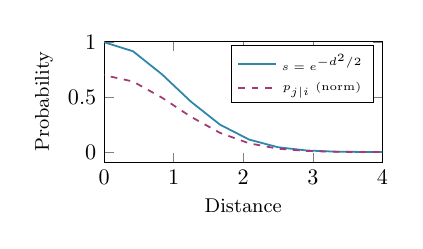
\begin{tikzpicture}[scale=0.8]
\begin{axis}[
    xlabel={\small Distance},
    ylabel={\small Probability},
    width=6cm, height=3.5cm,
    xmin=0, xmax=4,
    legend pos=north east,
    legend style={font=\tiny}
]
\addplot[highDcolor, thick] {exp(-x^2/2)};
\addlegendentry{$s = e^{-d^2/2}$}
\addplot[lowDcolor, thick, dashed] {0.7*exp(-x^2/2)};
\addlegendentry{$p_{j|i}$ (norm)}
\end{axis}
\end{tikzpicture}

\small
$d = 1$: $s \approx 0.606$\\
$d = 2$: $s \approx 0.135$
\end{columns}
\end{frame}

% SLIDE 7 (FIXED)
\begin{frame}
\frametitle{Computing Conditional Probabilities}
\begin{columns}[T]
\column{0.45\textwidth}
\textbf{Example: 3 points}
\begin{center}
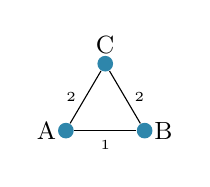
\begin{tikzpicture}[scale=0.5]
\node[circle,fill=highDcolor,inner sep=2pt] (A) at (0,0) {};
\node[circle,fill=highDcolor,inner sep=2pt] (B) at (2,0) {};
\node[circle,fill=highDcolor,inner sep=2pt] (C) at (1,1.7) {};
\draw (A) -- node[below] {\tiny 1} (B);
\draw (B) -- node[right] {\tiny 2} (C);
\draw (C) -- node[left] {\tiny 2} (A);
\node[left] at (A) {\small A};
\node[right] at (B) {\small B};
\node[above] at (C) {\small C};
\end{tikzpicture}
\end{center}

\textbf{With $\sigma_A = 1$:}\\
$s_{AB} = e^{-1/2} \approx 0.606$\\
$s_{AC} = e^{-2} \approx 0.135$\\
Sum = 0.741

\vspace{0.2cm}
$p_{B|A} = 0.606/0.741 \approx 0.82$\\
$p_{C|A} = 0.135/0.741 \approx 0.18$

\column{0.55\textwidth}
\textbf{Key Properties:}
\begin{itemize}
\small
\item $\sum_j p_{j|i} = 1$ (normalized)
\item $p_{j|i} \neq p_{i|j}$ (asymmetric)
\item Close points: high probability
\item Far points: nearly zero
\end{itemize}

\vspace{0.2cm}
\textbf{Adaptive $\sigma$:}
\begin{center}
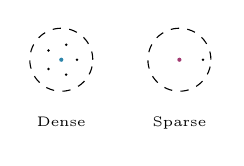
\begin{tikzpicture}[scale=0.5]
% Dense
\draw[dashed] (0,0) circle (0.8);
\fill[highDcolor] (0,0) circle (1.5pt);
\foreach \i in {1,...,5} {
    \pgfmathsetmacro{\angle}{72*\i}
    \fill ({0.4*cos(\angle)},{0.4*sin(\angle)}) circle (1pt);
}
\node[below] at (0,-1.2) {\tiny Dense};

% Sparse
\begin{scope}[shift={(3,0)}]
\draw[dashed] (0,0) circle (0.8);
\fill[lowDcolor] (0,0) circle (1.5pt);
\fill (0.6,0) circle (1pt);
\node[below] at (0,-1.2) {\tiny Sparse};
\end{scope}
\end{tikzpicture}
\end{center}
\end{columns}
\end{frame}

% SLIDE 8: Perplexity
\begin{frame}
\frametitle{Perplexity: Setting $\sigma_i$}
\begin{columns}[T]
\column{0.45\textwidth}
\textbf{Definition:}\\
Perplexity = $2^{H(P_i)}$\\
where $H(P_i) = -\sum_j p_{j|i} \log_2 p_{j|i}$

\vspace{0.3cm}
\textbf{Interpretation:}\\
Effective number of neighbors

\vspace{0.3cm}
\textbf{Algorithm:}
\begin{itemize}
\small
\item User sets perplexity (5-50)
\item Binary search finds $\sigma_i$
\item Each point gets its own $\sigma_i$
\end{itemize}

\column{0.55\textwidth}
\textbf{Example: Perplexity = 3}
\begin{center}
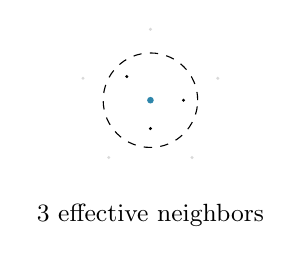
\begin{tikzpicture}[scale=0.6]
\fill[highDcolor] (0,0) circle (2pt);
\draw[dashed] (0,0) circle (1);
\fill (0.7,0) circle (1pt);
\fill (-0.5,0.5) circle (1pt);
\fill (0,-0.6) circle (1pt);
\foreach \i in {1,...,5} {
    \pgfmathsetmacro{\angle}{72*\i+90}
    \fill[gray!30] ({1.5*cos(\angle)},{1.5*sin(\angle)}) circle (1pt);
}
\node[below] at (0,-2) {\small 3 effective neighbors};
\end{tikzpicture}
\end{center}

\textbf{Typical values:}\\
Small data: perplexity = 5-30\\
Large data: perplexity = 30-50
\end{columns}
\end{frame}

% SLIDE 9: SNE Objective
\begin{frame}
\frametitle{SNE Objective Function}
\begin{columns}[T]
\column{0.5\textwidth}
\textbf{Kullback-Leibler divergence:}
$$C = \sum_i KL(P_i||Q_i)$$
$$= \sum_i \sum_j p_{j|i} \log\frac{p_{j|i}}{q_{j|i}}$$

\vspace{0.3cm}
\textbf{What KL measures:}
\begin{itemize}
\small
\item Info lost using $Q$ for $P$
\item Asymmetric penalty
\item Focus on preserving neighbors
\end{itemize}

\column{0.5\textwidth}
\textbf{Penalty structure:}
\begin{center}
\small
\begin{tabular}{|c|c|c|}
\hline
$p_{j|i}$ & $q_{j|i}$ & Cost \\
\hline
Large & Small & \textcolor{red}{High} \\
Small & Large & \textcolor{blue}{Low} \\
\hline
\end{tabular}
\end{center}

\vspace{0.3cm}
\textbf{Optimization:}\\
Gradient descent on $\mathbf{Y}$
$$\frac{\partial C}{\partial \mathbf{y}_i} = 2\sum_j (p_{j|i} - q_{j|i} + p_{i|j} - q_{i|j})(\mathbf{y}_i - \mathbf{y}_j)$$
\end{columns}
\end{frame}

% SLIDE 10: Why SNE Fails
\begin{frame}
\frametitle{Why SNE Fails: Crowding in Optimization}
\begin{columns}[T]
\column{0.5\textwidth}
\textbf{The Problem:}
\begin{itemize}
\small
\item Gaussian decay: $e^{-d^2}$
\item Too steep for moderate distances
\item Forces all points together
\end{itemize}

\vspace{0.3cm}
\textbf{Example:}\\
\small
Distance 2 vs 4:\\
$e^{-4}/e^{-16} = e^{12} \approx 162,754$\\
Ratio too extreme!

\vspace{0.3cm}
\textbf{Result:} Points collapse to center

\column{0.5\textwidth}
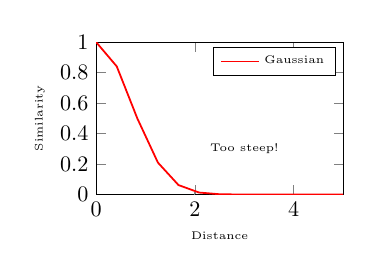
\begin{tikzpicture}[scale=0.8]
\begin{axis}[
    xlabel={\tiny Distance},
    ylabel={\tiny Similarity},
    width=5.5cm, height=4cm,
    xmin=0, xmax=5,
    ymin=0, ymax=1,
    legend pos=north east,
    legend style={font=\tiny}
]
\addplot[red, thick] {exp(-x^2)};
\addlegendentry{Gaussian}
\draw[dashed,gray] (axis cs:2,0) -- (axis cs:2,0.018);
\draw[dashed,gray] (axis cs:4,0) -- (axis cs:4,0.000003);
\node[font=\tiny] at (axis cs:3,0.3) {Too steep!};
\end{axis}
\end{tikzpicture}
\end{columns}
\end{frame}

% SLIDE 11: t-Distribution Solution
\begin{frame}
\frametitle{The t-Distribution Solution}
\begin{columns}[T]
\column{0.45\textwidth}
\textbf{Key Innovation:}\\
Replace Gaussian with Student-t (df=1)

\vspace{0.3cm}
\textbf{In low-D space:}
$$q_{ij} \propto (1 + \|\mathbf{y}_i - \mathbf{y}_j\|^2)^{-1}$$

\vspace{0.3cm}
\textbf{Heavy tails:}
\begin{itemize}
\small
\item More room for moderate distances
\item Alleviates crowding
\item Better separation
\end{itemize}

\column{0.55\textwidth}
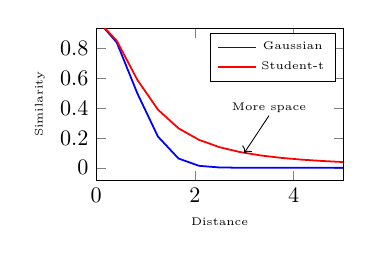
\begin{tikzpicture}[scale=0.8]
\begin{axis}[
    xlabel={\tiny Distance},
    ylabel={\tiny Similarity},
    width=5.5cm, height=4cm,
    xmin=0, xmax=5,
    legend pos=north east,
    legend style={font=\tiny}
]
\addplot[blue, thick] {exp(-x^2)};
\addlegendentry{Gaussian}
\addplot[red, thick] {1/(1+x^2)};
\addlegendentry{Student-t}
\node[font=\tiny] at (axis cs:3.5,0.4) {More space};
\draw[->] (axis cs:3.5,0.35) -- (axis cs:3,0.1);
\end{axis}
\end{tikzpicture}

\textbf{Ratio at d=2 vs d=4:}\\
\small t-dist: $(1+4)/(1+16) \approx 0.29$\\
\small Gaussian: $e^{-4}/e^{-16} \approx 162,754$
\end{columns}
\end{frame}

% SLIDE 12: Symmetric SNE
\begin{frame}
\frametitle{Symmetric t-SNE: The Final Form}
\begin{columns}[T]
\column{0.5\textwidth}
\textbf{Symmetrization:}
$$p_{ij} = \frac{p_{j|i} + p_{i|j}}{2n}$$
$$q_{ij} = \frac{(1+\|\mathbf{y}_i-\mathbf{y}_j\|^2)^{-1}}{\sum_{k \neq l}(1+\|\mathbf{y}_k-\mathbf{y}_l\|^2)^{-1}}$$

\vspace{0.3cm}
\textbf{Benefits:}
\begin{itemize}
\small
\item Simpler gradients
\item Better outlier handling  
\item Single KL divergence
\end{itemize}

\column{0.5\textwidth}
\textbf{Final objective:}
$$C = KL(P||Q) = \sum_{ij} p_{ij} \log\frac{p_{ij}}{q_{ij}}$$

\vspace{0.3cm}
\textbf{Gradient:}
$$\frac{\partial C}{\partial \mathbf{y}_i} = 4\sum_j (p_{ij} - q_{ij})F_{ij}(\mathbf{y}_i - \mathbf{y}_j)$$
where $F_{ij} = (1 + \|\mathbf{y}_i - \mathbf{y}_j\|^2)^{-1}$

\vspace{0.2cm}
This is t-SNE!
\end{columns}
\end{frame}

% SLIDE 13: Understanding the Gradient
\begin{frame}
\frametitle{Understanding the Gradient: Forces}
\begin{columns}[T]
\column{0.5\textwidth}
\textbf{Gradient as forces:}
$$\frac{\partial C}{\partial \mathbf{y}_i} = 4\sum_j (p_{ij} - q_{ij})F_{ij}(\mathbf{y}_i - \mathbf{y}_j)$$

\textbf{Two components:}
\begin{itemize}
\small
\item $(p_{ij} - q_{ij})$: strength
\item $(\mathbf{y}_i - \mathbf{y}_j)$: direction
\end{itemize}

\vspace{0.3cm}
\textbf{Interpretation:}
\begin{itemize}
\small
\item $p_{ij} > q_{ij}$: attract
\item $p_{ij} < q_{ij}$: repel
\end{itemize}

\column{0.5\textwidth}
\begin{center}
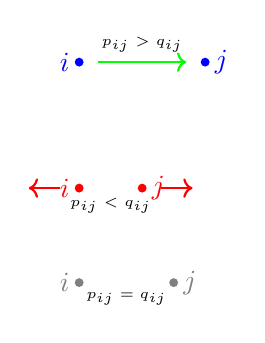
\begin{tikzpicture}[scale=0.8]
% Attraction
\fill[blue] (0,1) circle (2pt) node[left] {$i$};
\fill[blue] (2,1) circle (2pt) node[right] {$j$};
\draw[->,thick,green] (0.3,1) -- (1.7,1);
\node[above] at (1,1) {\tiny $p_{ij} > q_{ij}$};

% Repulsion
\fill[red] (0,-1) circle (2pt) node[left] {$i$};
\fill[red] (1,-1) circle (2pt) node[right] {$j$};
\draw[->,thick,red] (-0.3,-1) -- (-0.8,-1);
\draw[->,thick,red] (1.3,-1) -- (1.8,-1);
\node[below] at (0.5,-1) {\tiny $p_{ij} < q_{ij}$};

% Balanced
\fill[gray] (0,-2.5) circle (2pt) node[left] {$i$};
\fill[gray] (1.5,-2.5) circle (2pt) node[right] {$j$};
\node[below] at (0.75,-2.5) {\tiny $p_{ij} = q_{ij}$};
\end{tikzpicture}
\end{center}

\textbf{Equilibrium:} Forces balance
\end{columns}
\end{frame}

% SLIDE 14: Optimization Algorithm
\begin{frame}
\frametitle{Optimization Algorithm}
\begin{columns}[T]
\column{0.5\textwidth}
\textbf{Gradient Descent with Momentum:}
\begin{itemize}
\small
\item Initialize: $\mathbf{Y} \sim \mathcal{N}(0, 10^{-4}I)$
\item Learning rate: $\eta = 200$
\item Momentum: $\alpha = 0.5$ (then 0.8)
\end{itemize}

\vspace{0.3cm}
\textbf{Update rule:}
$$\mathcal{Y}^{(t)} = \mathcal{Y}^{(t-1)} + \eta \frac{\partial C}{\partial \mathcal{Y}} + \alpha(\mathcal{Y}^{(t-1)} - \mathcal{Y}^{(t-2)})$$

\vspace{0.3cm}
\textbf{Early exaggeration:}\\
\small Multiply all $p_{ij}$ by 4 for first 250 iterations

\column{0.5\textwidth}
\textbf{Typical schedule:}
\begin{center}
\small
\begin{tabular}{|l|c|}
\hline
Iterations & Setting \\
\hline
1-250 & Exaggeration = 4 \\
& $\alpha = 0.5$ \\
\hline
251-1000 & No exaggeration \\
& $\alpha = 0.8$ \\
\hline
\end{tabular}
\end{center}

\vspace{0.3cm}
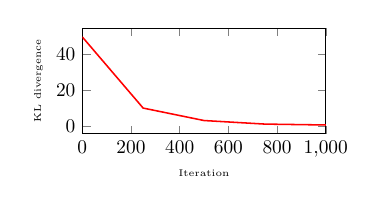
\begin{tikzpicture}[scale=0.7]
\begin{axis}[
    xlabel={\tiny Iteration},
    ylabel={\tiny KL divergence},
    width=6cm, height=3.5cm,
    xmin=0, xmax=1000
]
\addplot[red, thick] coordinates {
    (0,50) (250,10) (500,3) (750,1) (1000,0.5)
};
\end{axis}
\end{tikzpicture}
\end{columns}
\end{frame}

% SLIDE 15: Computational Complexity
\begin{frame}
\frametitle{Computational Complexity}
\begin{columns}[T]
\column{0.5\textwidth}
\textbf{Naive implementation:}
\begin{itemize}
\small
\item Computing all $q_{ij}$: $O(n^2)$
\item Per iteration: $O(n^2)$
\item 1000 iterations: $O(1000n^2)$
\end{itemize}

\vspace{0.3cm}
\textbf{Memory: $O(n^2)$ for $P$ matrix}

\vspace{0.3cm}
\textbf{Example times:}
\begin{center}
\small
\begin{tabular}{|c|c|}
\hline
$n$ & Time \\
\hline
1,000 & 30 sec \\
10,000 & 50 min \\
100,000 & 3+ days \\
\hline
\end{tabular}
\end{center}

\column{0.5\textwidth}
\textbf{Barnes-Hut t-SNE:}
\begin{itemize}
\small
\item Uses quad/oct-trees
\item Approximates far interactions
\item Complexity: $O(n \log n)$
\item Accuracy parameter $\theta$
\end{itemize}

\vspace{0.3cm}
\begin{center}
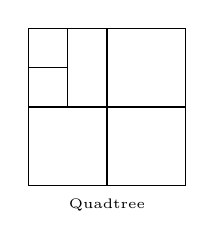
\begin{tikzpicture}[scale=0.5]
% Quadtree illustration
\draw (0,0) rectangle (4,4);
\draw (2,0) -- (2,4);
\draw (0,2) -- (4,2);
\draw (1,2) -- (1,4);
\draw (0,3) -- (1,3);
\node at (2,-0.5) {\tiny Quadtree};
\end{tikzpicture}
\end{center}

\textbf{Speedup:} 100x for large $n$
\end{columns}
\end{frame}

% SLIDE 16: Practical Implementation Tips
\begin{frame}
\frametitle{Practical Implementation Tips}
\begin{columns}[T]
\column{0.5\textwidth}
\textbf{Preprocessing:}
\begin{enumerate}
\small
\item Center data: mean = 0
\item Scale: unit variance
\item PCA to 50 dims (if $d > 50$)
\item Remove duplicates
\end{enumerate}

\vspace{0.3cm}
\textbf{Parameter selection:}
\begin{itemize}
\small
\item Perplexity: try 5, 30, 50
\item Learning rate: $n/12$ or 200
\item Iterations: min 1000
\end{itemize}

\column{0.5\textwidth}
\textbf{Common pitfalls:}
\begin{itemize}
\small
\item Too few iterations
\item Single perplexity value
\item Not checking convergence
\item Interpreting distances
\end{itemize}

\vspace{0.3cm}
\textbf{Best practice:}\\
\small Run 5 times with different seeds\\
Check stability of clusters
\end{columns}
\end{frame}

% SLIDE 17: Convergence and Validation
\begin{frame}
\frametitle{Convergence and Validation}
\begin{columns}[T]
\column{0.5\textwidth}
\textbf{Monitor convergence:}
\begin{itemize}
\small
\item KL divergence decrease
\item Gradient norm $< 10^{-7}$
\item Visual stability
\end{itemize}

\vspace{0.3cm}
\textbf{Validation strategies:}
\begin{enumerate}
\small
\item Known labels: check separation
\item Multiple runs: consistency
\item Different perplexities
\item Subset analysis
\end{enumerate}

\column{0.5\textwidth}
\begin{center}
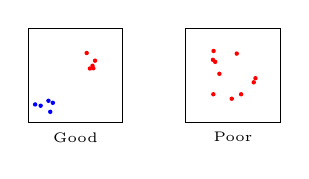
\begin{tikzpicture}[scale=0.4]
% Good embedding
\begin{scope}
\draw (0,0) rectangle (3,3);
\foreach \i in {1,...,5} {
    \pgfmathsetmacro{\x}{0.5+rand*0.3}
    \pgfmathsetmacro{\y}{0.5+rand*0.3}
    \fill[blue] (\x,\y) circle (2pt);
}
\foreach \i in {1,...,5} {
    \pgfmathsetmacro{\x}{2+rand*0.3}
    \pgfmathsetmacro{\y}{2+rand*0.3}
    \fill[red] (\x,\y) circle (2pt);
}
\node[below] at (1.5,0) {\tiny Good};
\end{scope}

% Bad embedding
\begin{scope}[shift={(5,0)}]
\draw (0,0) rectangle (3,3);
\foreach \i in {1,...,10} {
    \pgfmathsetmacro{\x}{1.5+rand*0.8}
    \pgfmathsetmacro{\y}{1.5+rand*0.8}
    \pgfmathsetmacro{\c}{rand}
    \ifnum \pgfmathresult > 0
        \fill[blue] (\x,\y) circle (2pt);
    \else
        \fill[red] (\x,\y) circle (2pt);
    \fi
}
\node[below] at (1.5,0) {\tiny Poor};
\end{scope}
\end{tikzpicture}
\end{center}

\textbf{Quality indicators:}\\
\small Clear clusters, stable across runs
\end{columns}
\end{frame}

% SLIDE 18: Worked Example - Setup
\begin{frame}
\frametitle{Complete Example: 5 Points}
\begin{columns}[T]
\column{0.5\textwidth}
\textbf{High-D data (simplified):}
\begin{center}
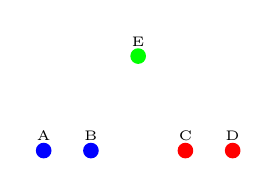
\begin{tikzpicture}[scale=0.6]
\node[circle,fill=blue,inner sep=2pt] (A) at (0,0) {};
\node[circle,fill=blue,inner sep=2pt] (B) at (1,0) {};
\node[circle,fill=red,inner sep=2pt] (C) at (3,0) {};
\node[circle,fill=red,inner sep=2pt] (D) at (4,0) {};
\node[circle,fill=green,inner sep=2pt] (E) at (2,2) {};
\node[above] at (A) {\tiny A};
\node[above] at (B) {\tiny B};
\node[above] at (C) {\tiny C};
\node[above] at (D) {\tiny D};
\node[above] at (E) {\tiny E};
\end{tikzpicture}
\end{center}

\textbf{Distance matrix:}
\begin{center}
\tiny
\begin{tabular}{c|ccccc}
  & A & B & C & D & E \\
\hline
A & 0 & 1 & 3 & 4 & 2.2 \\
B & 1 & 0 & 2 & 3 & 1.4 \\
C & 3 & 2 & 0 & 1 & 1.4 \\
D & 4 & 3 & 1 & 0 & 2.2 \\
E & 2.2 & 1.4 & 1.4 & 2.2 & 0 \\
\end{tabular}
\end{center}

\column{0.5\textwidth}
\textbf{Goal:}\\
Map to 2D preserving structure

\vspace{0.3cm}
\textbf{Expected result:}
\begin{itemize}
\small
\item A-B close (blue cluster)
\item C-D close (red cluster)
\item E somewhat separate
\end{itemize}

\vspace{0.3cm}
\textbf{Parameters:}
\begin{itemize}
\small
\item Perplexity = 2
\item Will find $\sigma_i$ for each point
\end{itemize}
\end{columns}
\end{frame}

% SLIDE 19: Computing P Matrix
\begin{frame}
\frametitle{Computing the P Matrix}
\begin{columns}[T]
\column{0.5\textwidth}
\textbf{Step 1: Find $\sigma_A$ (perp = 2)}

With $\sigma_A = 1.0$:
\begin{itemize}
\small
\item $s_{AB} = e^{-0.5} = 0.606$
\item $s_{AC} = e^{-4.5} = 0.011$
\item $s_{AD} = e^{-8} = 0.0003$
\item $s_{AE} = e^{-2.42} = 0.089$
\end{itemize}

Perplexity check: $2^H \approx 1.8$ ✓

\vspace{0.2cm}
\textbf{Normalize:}
\begin{itemize}
\small
\item $p_{B|A} = 0.606/0.706 = 0.858$
\item $p_{C|A} = 0.011/0.706 = 0.016$
\item $p_{D|A} = 0.0003/0.706 = 0.0004$
\item $p_{E|A} = 0.089/0.706 = 0.126$
\end{itemize}

\column{0.5\textwidth}
\textbf{Step 2: Symmetrize}
$$p_{ij} = \frac{p_{j|i} + p_{i|j}}{2n}$$

\textbf{Final P matrix (×1000):}
\begin{center}
\tiny
\begin{tabular}{c|ccccc}
  & A & B & C & D & E \\
\hline
A & 0 & 86 & 2 & 0.1 & 15 \\
B & 86 & 0 & 12 & 2 & 40 \\
C & 2 & 12 & 0 & 86 & 40 \\
D & 0.1 & 2 & 86 & 0 & 15 \\
E & 15 & 40 & 40 & 15 & 0 \\
\end{tabular}
\end{center}

Note: A-B and C-D have high $p_{ij}$
\end{columns}
\end{frame}

% SLIDE 20: Initial Embedding
\begin{frame}
\frametitle{Initial Embedding and Q Matrix}
\begin{columns}[T]
\column{0.5\textwidth}
\textbf{Random initialization:}
\begin{center}
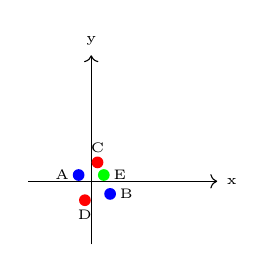
\begin{tikzpicture}[scale=0.8]
\draw[->] (-1,0) -- (2,0) node[right] {\tiny x};
\draw[->] (0,-1) -- (0,2) node[above] {\tiny y};
\node[circle,fill=blue,inner sep=1.5pt] (A) at (-0.2,0.1) {};
\node[circle,fill=blue,inner sep=1.5pt] (B) at (0.3,-0.2) {};
\node[circle,fill=red,inner sep=1.5pt] (C) at (0.1,0.3) {};
\node[circle,fill=red,inner sep=1.5pt] (D) at (-0.1,-0.3) {};
\node[circle,fill=green,inner sep=1.5pt] (E) at (0.2,0.1) {};
\node[left] at (A) {\tiny A};
\node[right] at (B) {\tiny B};
\node[above] at (C) {\tiny C};
\node[below] at (D) {\tiny D};
\node[right] at (E) {\tiny E};
\end{tikzpicture}
\end{center}

All points near origin\\
(random $\sim \mathcal{N}(0, 10^{-4})$)

\column{0.5\textwidth}
\textbf{Compute Q matrix:}
$$q_{ij} = \frac{(1+\|\mathbf{y}_i-\mathbf{y}_j\|^2)^{-1}}{\sum_{k<l}(1+\|\mathbf{y}_k-\mathbf{y}_l\|^2)^{-1}}$$

\textbf{Initial Q (×1000):}
\begin{center}
\tiny
\begin{tabular}{c|ccccc}
  & A & B & C & D & E \\
\hline
A & 0 & 18 & 22 & 21 & 19 \\
B & 18 & 0 & 19 & 23 & 20 \\
C & 22 & 19 & 0 & 18 & 21 \\
D & 21 & 23 & 18 & 0 & 19 \\
E & 19 & 20 & 21 & 19 & 0 \\
\end{tabular}
\end{center}

Nearly uniform! (all $\sim$ 20)
\end{columns}
\end{frame}

% SLIDE 21: First Optimization Step
\begin{frame}
\frametitle{First Optimization Step}
\begin{columns}[T]
\column{0.5\textwidth}
\textbf{Compute gradients:}

For point A:
$$\frac{\partial C}{\partial \mathbf{y}_A} = 4\sum_j (p_{Aj} - q_{Aj})F_{Aj}(\mathbf{y}_A - \mathbf{y}_j)$$

\textbf{Forces on A:}
\begin{itemize}
\small
\item From B: $(86-18) \times$ attract
\item From C: $(2-22) \times$ repel  
\item From D: $(0.1-21) \times$ repel
\item From E: $(15-19) \times$ repel
\end{itemize}

Result: A moves toward B

\column{0.5\textwidth}
\textbf{After 1 iteration:}
\begin{center}
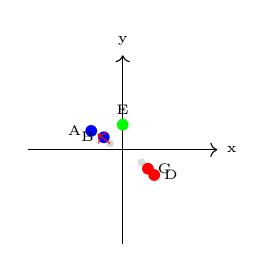
\begin{tikzpicture}[scale=0.8]
\draw[->] (-1.5,0) -- (1.5,0) node[right] {\tiny x};
\draw[->] (0,-1.5) -- (0,1.5) node[above] {\tiny y};
% Old positions (faded)
\node[circle,fill=gray!30,inner sep=1pt] at (-0.2,0.1) {};
\node[circle,fill=gray!30,inner sep=1pt] at (0.3,-0.2) {};
% New positions
\node[circle,fill=blue,inner sep=1.5pt] (A) at (-0.5,0.3) {};
\node[circle,fill=blue,inner sep=1.5pt] (B) at (-0.3,0.2) {};
\node[circle,fill=red,inner sep=1.5pt] (C) at (0.4,-0.3) {};
\node[circle,fill=red,inner sep=1.5pt] (D) at (0.5,-0.4) {};
\node[circle,fill=green,inner sep=1.5pt] (E) at (0,0.4) {};
\draw[->,red] (-0.2,0.1) -- (-0.4,0.25);
\node[left] at (A) {\tiny A};
\node[left] at (B) {\tiny B};
\node[right] at (C) {\tiny C};
\node[right] at (D) {\tiny D};
\node[above] at (E) {\tiny E};
\end{tikzpicture}
\end{center}

Clusters beginning to form!
\end{columns}
\end{frame}

% SLIDE 22: Effect of Perplexity
\begin{frame}
\frametitle{Effect of Perplexity}
\begin{columns}[T]
\column{0.3\textwidth}
\textbf{Perplexity = 1}
\begin{center}
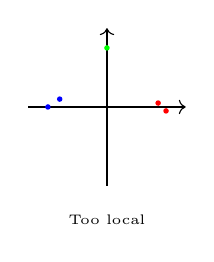
\begin{tikzpicture}[scale=0.5]
\draw[->] (-2,0) -- (2,0);
\draw[->] (0,-2) -- (0,2);
\fill[blue] (-1.5,0) circle (2pt);
\fill[blue] (-1.2,0.2) circle (2pt);
\fill[red] (1.3,0.1) circle (2pt);
\fill[red] (1.5,-0.1) circle (2pt);
\fill[green] (0,1.5) circle (2pt);
\node[below] at (0,-2.5) {\tiny Too local};
\end{tikzpicture}
\end{center}

\column{0.3\textwidth}
\textbf{Perplexity $=$ 2}
\begin{center}
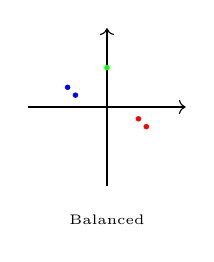
\begin{tikzpicture}[scale=0.5]
\draw[->] (-2,0) -- (2,0);
\draw[->] (0,-2) -- (0,2);
\fill[blue] (-1,0.5) circle (2pt);
\fill[blue] (-0.8,0.3) circle (2pt);
\fill[red] (0.8,-0.3) circle (2pt);
\fill[red] (1,-0.5) circle (2pt);
\fill[green] (0,1) circle (2pt);
\node[below] at (0,-2.5) {\tiny Balanced};
\end{tikzpicture}
\end{center}

\column{0.4\textwidth}
\textbf{Perplexity $=$ 4}
\begin{center}
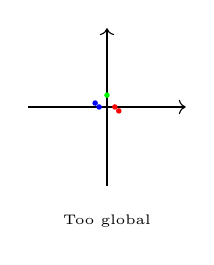
\begin{tikzpicture}[scale=0.5]
\draw[->] (-2,0) -- (2,0);
\draw[->] (0,-2) -- (0,2);
\fill[blue] (-0.3,0.1) circle (2pt);
\fill[blue] (-0.2,0) circle (2pt);
\fill[red] (0.2,0) circle (2pt);
\fill[red] (0.3,-0.1) circle (2pt);
\fill[green] (0,0.3) circle (2pt);
\node[below] at (0,-2.5) {\tiny Too global};
\end{tikzpicture}
\end{center}

\textbf{Rule:} 5 $\leq$ Perplexity $\leq$ 50
\end{columns}
\end{frame}

% SLIDE 23: Real Application - MNIST
\begin{frame}
\frametitle{Real Application: MNIST Digits}
\begin{columns}[T]
\column{0.5\textwidth}
\textbf{Dataset:}
\begin{itemize}
\small
\item 60,000 handwritten digits
\item 28×28 pixels = 784 dimensions
\item 10 classes (0-9)
\end{itemize}

\vspace{0.3cm}
\textbf{t-SNE settings:}
\begin{itemize}
\small
\item PCA to 50D first
\item Perplexity = 30
\item 1000 iterations
\end{itemize}

\vspace{0.3cm}
\textbf{What we see:}
\begin{itemize}
\small
\item Clear digit clusters
\item Similar digits nearby
\item 4-9-7 often close
\item 0-6 sometimes overlap
\end{itemize}

\column{0.5\textwidth}
\begin{center}
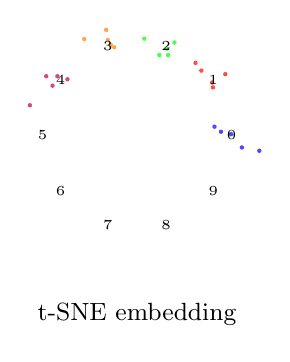
\begin{tikzpicture}[scale=0.8]
% Simplified MNIST visualization
\foreach \i in {0,...,9} {
    \pgfmathsetmacro{\angle}{36*\i}
    \pgfmathsetmacro{\r}{1.5}
    \coordinate (c\i) at ({\r*cos(\angle)},{\r*sin(\angle)});
}
% Clusters
\foreach \j in {1,...,5} {
    \pgfmathsetmacro{\noise}{0.2*rand}
    \fill[blue!70] ($(c0)+(0.1*\j*rand,0.1*\j*rand)$) circle (1pt);
    \fill[red!70] ($(c1)+(0.1*\j*rand,0.1*\j*rand)$) circle (1pt);
    \fill[green!70] ($(c2)+(0.1*\j*rand,0.1*\j*rand)$) circle (1pt);
    \fill[orange!70] ($(c3)+(0.1*\j*rand,0.1*\j*rand)$) circle (1pt);
    \fill[purple!70] ($(c4)+(0.1*\j*rand,0.1*\j*rand)$) circle (1pt);
}
\node at (c0) {\tiny 0};
\node at (c1) {\tiny 1};
\node at (c2) {\tiny 2};
\node at (c3) {\tiny 3};
\node at (c4) {\tiny 4};
\node at (c5) {\tiny 5};
\node at (c6) {\tiny 6};
\node at (c7) {\tiny 7};
\node at (c8) {\tiny 8};
\node at (c9) {\tiny 9};
\node[below] at (0,-2.5) {\small t-SNE embedding};
\end{tikzpicture}
\end{center}
\end{columns}
\end{frame}

% SLIDE 24: t-SNE vs PCA
\begin{frame}
\frametitle{t-SNE vs PCA: Same Data}
\begin{columns}[T]
\column{0.5\textwidth}
\textbf{PCA (linear):}
\begin{center}
\begin{tikzpicture}[scale=0.6]
\draw[->] (-2,0) -- (2,0) node[right] {\tiny PC1};
\draw[->] (0,-2) -- (0,2) node[above] {\tiny PC2};
% Mixed clusters
\foreach \i in {1,...,30} {
    \pgfmathsetmacro{\x}{2*rand}
    \pgfmathsetmacro{\y}{2*rand}
    \pgfmathsetmacro{\c}{random(0,2)}
    \ifnum\c=0
        \fill[blue!60] (\x,\y) circle (1pt);
    \else\ifnum\c=1
        \fill[red!60] (\x,\y) circle (1pt);
    \else
        \fill[green!60] (\x,\y) circle (1pt);
    \fi\fi
}
\end{tikzpicture}
\end{center}

\begin{itemize}
\small
\item Maximizes variance
\item Linear projection
\item Overlapping clusters
\item Fast computation
\end{itemize}

\column{0.5\textwidth}
\textbf{t-SNE (nonlinear):}
\begin{center}
\begin{tikzpicture}[scale=0.6]
\draw[->] (-2,0) -- (2,0) node[right] {\tiny Dim1};
\draw[->] (0,-2) -- (0,2) node[above] {\tiny Dim2};
% Separated clusters
\foreach \i in {1,...,10} {
    \pgfmathsetmacro{\x}{-1+0.3*rand}
    \pgfmathsetmacro{\y}{1+0.3*rand}
    \fill[blue!80] (\x,\y) circle (1pt);
}
\foreach \i in {1,...,10} {
    \pgfmathsetmacro{\x}{1+0.3*rand}
    \pgfmathsetmacro{\y}{1+0.3*rand}
    \fill[red!80] (\x,\y) circle (1pt);
}
\foreach \i in {1,...,10} {
    \pgfmathsetmacro{\x}{0+0.3*rand}
    \pgfmathsetmacro{\y}{-1+0.3*rand}
    \fill[green!80] (\x,\y) circle (1pt);
}
\end{tikzpicture}
\end{center}

\begin{itemize}
\small
\item Preserves neighborhoods
\item Nonlinear mapping
\item Clear clusters
\item Slow computation
\end{itemize}
\end{columns}
\end{frame}

% SLIDE 25: Interpretation Pitfalls
\begin{frame}
\frametitle{Interpretation Pitfalls}
\begin{columns}[T]
\column{0.5\textwidth}
\textbf{What NOT to trust:}

\textbf{1. Distances between clusters}
\begin{center}
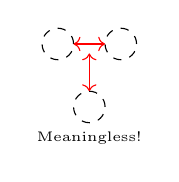
\begin{tikzpicture}[scale=0.4]
\draw[dashed] (-1,0) circle (0.5);
\draw[dashed] (1,0) circle (0.5);
\draw[dashed] (0,-2) circle (0.5);
\draw[<->,red] (-0.5,0) -- (0.5,0);
\draw[<->,red] (0,-0.3) -- (0,-1.5);
\node at (0,-3) {\tiny Meaningless!};
\end{tikzpicture}
\end{center}

\textbf{2. Cluster sizes}
\begin{center}
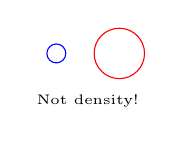
\begin{tikzpicture}[scale=0.4]
\draw[blue] (0,0) circle (0.3);
\draw[red] (2,0) circle (0.8);
\node at (1,-1.5) {\tiny Not density!};
\end{tikzpicture}
\end{center}

\column{0.5\textwidth}
\textbf{What TO trust:}

\textbf{1. Local structure}
\begin{itemize}
\small
\item Points close → similar
\item Within-cluster relationships
\end{itemize}

\textbf{2. Cluster existence}
\begin{itemize}
\small
\item Clear separations meaningful
\item But validate with other methods
\end{itemize}

\vspace{0.3cm}
\textbf{Remember:}\\
\small t-SNE creates a useful map,\\
not a perfect representation
\end{columns}
\end{frame}

% SLIDE 26: When t-SNE Fails
\begin{frame}
\frametitle{When t-SNE Can Mislead}
\begin{columns}[T]
\column{0.5\textwidth}
\textbf{Scenario 1: No real clusters}

Random uniform data can show fake clusters!

\begin{center}
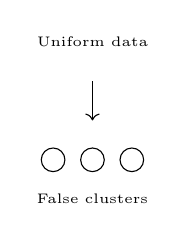
\begin{tikzpicture}[scale=0.5]
\node at (0,2) {\tiny Uniform data};
\draw[->] (0,1) -- (0,0);
\draw (0,-1) circle (0.3);
\draw (1,-1) circle (0.3);
\draw (-1,-1) circle (0.3);
\node at (0,-2) {\tiny False clusters};
\end{tikzpicture}
\end{center}

\textbf{Scenario 2: Wrong perplexity}
\begin{itemize}
\small
\item Too low: fragments clusters
\item Too high: merges clusters
\end{itemize}

\column{0.5\textwidth}
\textbf{Scenario 3: Insufficient iterations}
\begin{center}
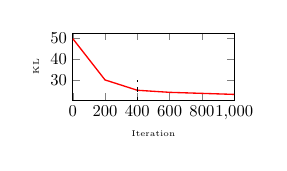
\begin{tikzpicture}[scale=0.6]
\begin{axis}[
    xlabel={\tiny Iteration},
    ylabel={\tiny KL},
    width=5cm, height=3cm,
    xmin=0, xmax=1000
]
\addplot[red, thick] coordinates {
    (0,50) (200,30) (400,25) (600,24) (800,23.5) (1000,23)
};
\draw[dashed] (axis cs:400,0) -- (axis cs:400,30);
\node at (axis cs:400,10) {\tiny Stop?};
\end{axis}
\end{tikzpicture}
\end{center}

\textbf{Solution:}
\begin{itemize}
\small
\item Multiple perplexities
\item Run to convergence
\item Multiple random seeds
\end{itemize}
\end{columns}
\end{frame}

% SLIDE 27: Validation Strategies
\begin{frame}
\frametitle{Validation Strategies}
\begin{columns}[T]
\column{0.5\textwidth}
\textbf{1. Stability check:}
\begin{itemize}
\small
\item Run 5-10 times
\item Different random seeds
\item Compare results
\end{itemize}

\textbf{2. Parameter sweep:}
\begin{itemize}
\small
\item Perplexity: 5, 10, 30, 50, 100
\item Look for consistent patterns
\end{itemize}

\textbf{3. Known structure:}
\begin{itemize}
\small
\item If labels exist, check separation
\item Silhouette score
\item Nearest neighbor preservation
\end{itemize}

\column{0.5\textwidth}
\textbf{4. Complementary methods:}
\begin{center}
\small
\begin{tabular}{|l|l|}
\hline
Method & Check \\
\hline
PCA & Global structure \\
UMAP & Alternative view \\
Clustering & Group validity \\
\hline
\end{tabular}
\end{center}

\vspace{0.3cm}
\textbf{Quality metrics:}
\begin{itemize}
\small
\item Trustworthiness: $T(k)$
\item Continuity: $C(k)$
\item KL divergence convergence
\end{itemize}

\textbf{Golden rule:}\\
\small Never trust a single t-SNE run!
\end{columns}
\end{frame}


% SLIDE 28: Non-convex Optimization
\begin{frame}
\frametitle{Non-convex Optimization Landscape}
\begin{columns}[T]
\column{0.5\textwidth}
\textbf{The Challenge:}
\begin{itemize}
\small
\item KL divergence is non-convex in $\mathbf{Y}$
\item Multiple local minima
\item Different initializations → different solutions
\end{itemize}

\vspace{0.3cm}
\textbf{Mathematical reason:}\\
\small
The function
$$q_{ij} = \frac{(1+\|\mathbf{y}_i-\mathbf{y}_j\|^2)^{-1}}{\sum_{k<l}(1+\|\mathbf{y}_k-\mathbf{y}_l\|^2)^{-1}}$$
is non-convex in $\mathbf{y}_i$

\vspace{0.3cm}
\textbf{Consequence:}\\
No guarantee of global optimum

\column{0.5\textwidth}
\begin{center}
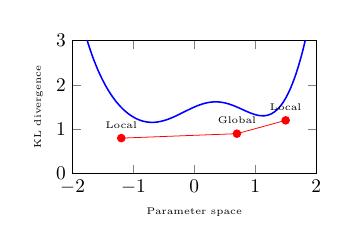
\begin{tikzpicture}[scale=0.7]
\begin{axis}[
    xlabel={\tiny Parameter space},
    ylabel={\tiny KL divergence},
    width=6cm, height=4cm,
    xmin=-2, xmax=2,
    ymin=0, ymax=3
]
\addplot[blue, thick, smooth, samples=100] {
    0.3*x^4 - 0.5*x^2 + 0.2*sin(deg(3*x)) + 1.5
};
\addplot[mark=*, red] coordinates {(-1.2,0.8) (0.7,0.9) (1.5,1.2)};
\node at (axis cs:-1.2,1.1) {\tiny Local};
\node at (axis cs:0.7,1.2) {\tiny Global};
\node at (axis cs:1.5,1.5) {\tiny Local};
\end{axis}
\end{tikzpicture}
\end{center}

\textbf{Solution:} Multiple runs
\end{columns}
\end{frame}

% SLIDE 29: Barnes-Hut Approximation
\begin{frame}
\frametitle{Barnes-Hut Approximation}
\begin{columns}[T]
\column{0.5\textwidth}
\textbf{The Idea:}
\begin{itemize}
\small
\item Group distant points
\item Treat as single point
\item Use tree structure
\end{itemize}

\vspace{0.3cm}
\textbf{Criterion:}
$$\frac{r_{\text{cell}}}{d_{\text{cell},i}} < \theta$$
where $\theta \approx 0.5$ (accuracy)

\vspace{0.3cm}
\textbf{Complexity:}
\begin{itemize}
\small
\item Naive: $O(n^2)$
\item Barnes-Hut: $O(n \log n)$
\end{itemize}

\column{0.5\textwidth}
\begin{center}
\begin{tikzpicture}[scale=0.6]
% Quadtree
\draw (0,0) rectangle (4,4);
\draw (2,0) -- (2,4);
\draw (0,2) -- (4,2);
\draw (1,2) -- (1,4);
\draw (0,3) -- (1,3);
% Points
\fill[blue] (0.5,3.5) circle (2pt);
\fill[blue] (0.3,3.3) circle (2pt);
\fill[red] (3,3) circle (2pt);
\fill[red] (3,1) circle (2pt);
\fill[green] (1.5,0.5) circle (2pt);
% Annotation
\draw[<-] (0.5,3) -- (-0.5,2);
\node[left] at (-0.5,2) {\tiny Grouped};
\draw[<-] (3,2) -- (5,2);
\node[right] at (5,2) {\tiny Individual};
\end{tikzpicture}
\end{center}

\textbf{Error bound:}\\
\small $|F_{\text{exact}} - F_{\text{approx}}| \leq \epsilon F_{\text{exact}}$
\end{columns}
\end{frame}

% SLIDE 30: Why Student-t Works
\begin{frame}
\frametitle{Mathematical Proof: Why Student-t?}
\begin{columns}[T]
\column{0.5\textwidth}
\textbf{Volume preservation:}

In $d$ dimensions, volume element:
$$dV_d = r^{d-1} dr \, d\Omega_{d-1}$$

For uniform distribution:
$$P(r) \propto r^{d-1}$$

\vspace{0.2cm}
\textbf{In high-D:}\\
\small Most volume at $r \approx \sqrt{d}$

\vspace{0.2cm}
\textbf{Student-t tail:}
$$t(r) \sim r^{-(d+1)}$$
Exactly compensates!

\column{0.5\textwidth}
\textbf{Mathematical argument:}

\small
Gaussian: $e^{-r^2} \cdot r^{d-1}$ peaks at $r = \sqrt{(d-1)/2}$

Student-t: $(1+r^2)^{-1} \cdot r$ is flatter

\vspace{0.3cm}
\textbf{Key ratio:}
$$\frac{q_{ij}}{q_{kl}} = \frac{1+\|\mathbf{y}_k-\mathbf{y}_l\|^2}{1+\|\mathbf{y}_i-\mathbf{y}_j\|^2}$$

Linear in squared distance!\\
(Gaussian is exponential)
\end{columns}
\end{frame}

% SLIDE 31: Manifold Learning Connection
\begin{frame}
\frametitle{Connection to Manifold Learning}
\begin{columns}[T]
\column{0.5\textwidth}
\textbf{Manifold hypothesis:}\\
\small High-D data lies on low-D manifold

\vspace{0.3cm}
\textbf{Methods comparison:}
\begin{center}
\tiny
\begin{tabular}{|l|l|}
\hline
Method & Preserves \\
\hline
Isomap & Geodesic distances \\
LLE & Local linear structure \\
Laplacian & Graph structure \\
t-SNE & Local probabilities \\
\hline
\end{tabular}
\end{center}

\vspace{0.3cm}
\textbf{t-SNE advantage:}\\
\small Adaptive bandwidth handles varying density

\column{0.5\textwidth}
\begin{center}
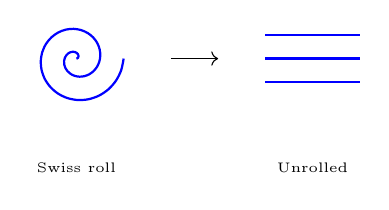
\begin{tikzpicture}[scale=0.6]
% Swiss roll illustration
\draw[thick,blue,domain=0:720,smooth,samples=50] 
    plot ({0.5*\x/360*cos(\x)},{0.5*\x/360*sin(\x)});
\node[below] at (0,-2) {\tiny Swiss roll};
\draw[->] (2,0) -- (3,0);
% Unrolled
\begin{scope}[shift={(5,0)}]
\draw[thick,blue] (-1,-0.5) -- (1,-0.5);
\draw[thick,blue] (-1,0) -- (1,0);
\draw[thick,blue] (-1,0.5) -- (1,0.5);
\node[below] at (0,-2) {\tiny Unrolled};
\end{scope}
\end{tikzpicture}
\end{center}

\textbf{Graph Laplacian view:}
$$\mathcal{L} = D - W$$
where $W_{ij} = p_{ij}$ (similarities)
\end{columns}
\end{frame}

% SLIDE 32: Theoretical Guarantees
\begin{frame}
\frametitle{Theoretical Guarantees and Limitations}
\begin{columns}[T]
\column{0.5\textwidth}
\textbf{What we DON'T have:}
\begin{itemize}
\small
\item Global convergence guarantee
\item Unique solution
\item Distance preservation bounds
\item Consistency as $n \to \infty$
\end{itemize}

\vspace{0.3cm}
\textbf{What we DO have:}
\begin{itemize}
\small
\item Local neighborhood preservation
\item Gradient convergence to local min
\item Empirical success
\end{itemize}

\column{0.5\textwidth}
\textbf{Open problems:}
\begin{enumerate}
\small
\item Optimal perplexity selection
\item Convergence rate analysis  
\item Approximation quality bounds
\item Statistical properties
\end{enumerate}

\vspace{0.3cm}
\textbf{Key limitation:}\\
\small No embedding quality guarantee\\
unlike PCA's variance explanation

\vspace{0.3cm}
\textbf{Bottom line:}\\
\small Powerful tool, but use carefully
\end{columns}
\end{frame}


% SLIDE 33: t-SNE vs UMAP
\begin{frame}
\frametitle{t-SNE vs UMAP}
\begin{columns}[T]
\column{0.5\textwidth}
\textbf{UMAP (2018):}
\begin{itemize}
\small
\item Based on topology theory
\item Fuzzy simplicial sets
\item Cross-entropy objective
\item Faster: $O(n^{1.14})$
\end{itemize}

\vspace{0.3cm}
\textbf{Mathematical difference:}\\
\small
UMAP: $q_{ij} = (1 + a\|\mathbf{y}_i-\mathbf{y}_j\|^{2b})^{-1}$\\
t-SNE: $q_{ij} = (1 + \|\mathbf{y}_i-\mathbf{y}_j\|^2)^{-1}$

\vspace{0.2cm}
Parameters $a,b$ learned from data

\column{0.5\textwidth}
\begin{center}
\small
\begin{tabular}{|l|c|c|}
\hline
Feature & t-SNE & UMAP \\
\hline
Speed & Slow & Fast \\
Global & No & Partial \\
Theory & Prob & Topo \\
Params & 1 & 4+ \\
Stable & No & More \\
\hline
\end{tabular}
\end{center}

\vspace{0.3cm}
\textbf{When to use which:}
\begin{itemize}
\small
\item t-SNE: Final visualization
\item UMAP: Exploration, large data
\end{itemize}
\end{columns}
\end{frame}

% SLIDE 34: Parametric t-SNE
\begin{frame}
\frametitle{Parametric t-SNE: Neural Network Approach}
\begin{columns}[T]
\column{0.5\textwidth}
\textbf{The Idea:}\\
Learn function $f_\theta: \mathbb{R}^d \to \mathbb{R}^2$

\vspace{0.3cm}
\textbf{Neural network:}
\begin{center}
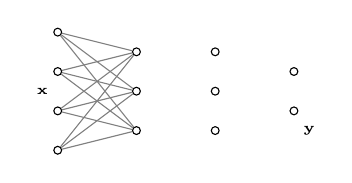
\begin{tikzpicture}[scale=0.5]
% Input layer
\foreach \i in {1,...,4} {
    \node[circle,draw,inner sep=1pt] (x\i) at (0,\i) {};
}
\node[left] at (0,2.5) {\tiny $\mathbf{x}$};
% Hidden layers
\foreach \i in {1,...,3} {
    \node[circle,draw,inner sep=1pt] (h1\i) at (2,\i+0.5) {};
}
\foreach \i in {1,...,3} {
    \node[circle,draw,inner sep=1pt] (h2\i) at (4,\i+0.5) {};
}
% Output
\foreach \i in {1,2} {
    \node[circle,draw,inner sep=1pt] (y\i) at (6,\i+1) {};
}
\node[right] at (6,1.5) {\tiny $\mathbf{y}$};
% Connections
\foreach \i in {1,...,4} {
    \foreach \j in {1,...,3} {
        \draw[gray] (x\i) -- (h1\j);
    }
}
\end{tikzpicture}
\end{center}

\textbf{Loss function:}
$$\mathcal{L} = KL(P||Q) + \lambda \|\theta\|^2$$

\column{0.5\textwidth}
\textbf{Advantages:}
\begin{itemize}
\small
\item Out-of-sample predictions
\item No need to store $\mathbf{Y}$
\item Can use mini-batches
\end{itemize}

\vspace{0.3cm}
\textbf{Training:}
\begin{enumerate}
\small
\item Sample batch of points
\item Compute $p_{ij}$ for batch
\item Forward pass: $\mathbf{y}_i = f_\theta(\mathbf{x}_i)$
\item Compute $q_{ij}$
\item Backprop KL gradient
\end{enumerate}

\vspace{0.3cm}
\textbf{Limitation:}\\
\small Less flexible than non-parametric
\end{columns}
\end{frame}

% SLIDE 35: Quality Metrics
\begin{frame}
\frametitle{Embedding Quality Metrics}
\begin{columns}[T]
\column{0.5\textwidth}
\textbf{1. Trustworthiness:}
$$T(k) = 1 - \frac{2}{nk(2n-3k-1)}\sum_i \sum_{j \in U_i^k} (r_{ij} - k)$$

\small Measures false neighbors

\vspace{0.3cm}
\textbf{2. Continuity:}
$$C(k) = 1 - \frac{2}{nk(2n-3k-1)}\sum_i \sum_{j \in V_i^k} (\hat{r}_{ij} - k)$$

\small Measures torn neighborhoods

\column{0.5\textwidth}
\textbf{3. Neighborhood preservation:}
$$NPR = \frac{1}{n}\sum_i \frac{|N_k(\mathbf{x}_i) \cap N_k(\mathbf{y}_i)|}{k}$$

\vspace{0.3cm}
\textbf{Example values:}
\begin{center}
\small
\begin{tabular}{|l|c|}
\hline
Metric & Good \\
\hline
$T(10)$ & $>$ 0.95 \\
$C(10)$ & $>$ 0.95 \\
NPR & $>$ 0.7 \\
\hline
\end{tabular}
\end{center}

\textbf{Visual check:}\\
\small Still most reliable!
\end{columns}
\end{frame}

% SLIDE 36: Recent Advances
\begin{frame}
\frametitle{Recent Advances (2020-2025)}
\begin{columns}[T]
\column{0.5\textwidth}
\textbf{1. FIt-SNE:}
\begin{itemize}
\small
\item FFT acceleration
\item Interpolation-based
\item 100x speedup
\end{itemize}

\vspace{0.3cm}
\textbf{2. openTSNE:}
\begin{itemize}
\small
\item Modular implementation
\item Custom objectives
\item Initialization options
\end{itemize}

\vspace{0.3cm}
\textbf{3. GPU-SNE:}
\begin{itemize}
\small
\item CUDA implementation
\item Millions of points
\item Real-time interaction
\end{itemize}

\column{0.5\textwidth}
\textbf{4. Dynamic t-SNE:}
\begin{center}
\begin{tikzpicture}[scale=0.5]
\foreach \t in {0,1,2} {
    \begin{scope}[shift={(\t*3,0)}]
    \draw[->] (-0.5,0) -- (0.5,0);
    \draw[->] (0,-0.5) -- (0,0.5);
    \node[below] at (0,-1) {\tiny $t=\t$};
    \fill[blue] (-0.2+0.1*\t,0.2) circle (1pt);
    \fill[red] (0.2-0.1*\t,-0.2) circle (1pt);
    \end{scope}
}
\end{tikzpicture}
\end{center}
For time-series embeddings

\vspace{0.3cm}
\textbf{5. Hierarchical t-SNE:}
\begin{itemize}
\small
\item Multi-scale visualization
\item Zoom in/out of clusters
\item Interactive exploration
\end{itemize}
\end{columns}
\end{frame}

% SLIDE 37: Software Implementation
\begin{frame}
\frametitle{Software and Implementation}
\begin{columns}[T]
\column{0.5\textwidth}
\textbf{Python:}
\begin{itemize}
\small
\item \texttt{sklearn.manifold.TSNE}
\item \texttt{openTSNE} (recommended)
\item \texttt{FIt-SNE}
\item \texttt{RAPIDS cuML} (GPU)
\end{itemize}

\vspace{0.3cm}
\textbf{R:}
\begin{itemize}
\small
\item \texttt{Rtsne} package
\item \texttt{tsne} package
\end{itemize}

\vspace{0.3cm}
\textbf{Best practices:}
\begin{itemize}
\small
\item Use PCA preprocessing
\item Set verbose=True
\item Save intermediate results
\end{itemize}

\column{0.5\textwidth}
\textbf{Typical workflow:}
\begin{enumerate}
\small
\item Load data
\item Standardize features
\item PCA to 50D
\item t-SNE with perp=30
\item Try perp=\{5,50,100\}
\item Validate clusters
\end{enumerate}

\vspace{0.3cm}
\textbf{Performance tips:}
\begin{itemize}
\small
\item Use float32, not float64
\item Barnes-Hut for $n > 5000$
\item GPU for $n > 50000$
\item Subsample if needed
\end{itemize}
\end{columns}
\end{frame}

% SLIDE 38: Biological Data Applications
\begin{frame}
\frametitle{Application: Single-Cell RNA Sequencing}
\begin{columns}[T]
\column{0.5\textwidth}
\textbf{The Challenge:}
\begin{itemize}
\small
\item 20,000+ genes (dimensions)
\item 10,000+ cells (points)
\item Sparse data (90\% zeros)
\item Technical noise
\end{itemize}

\vspace{0.3cm}
\textbf{Preprocessing:}
\begin{enumerate}
\small
\item Log normalization
\item Highly variable genes
\item PCA to 50 components
\item t-SNE on PCA space
\end{enumerate}

\vspace{0.3cm}
\textbf{Reveals:} Cell types, states, trajectories

\column{0.5\textwidth}
\begin{center}
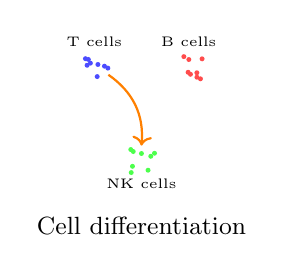
\begin{tikzpicture}[scale=0.6]
% Cell types visualization
\foreach \i in {1,...,8} {
    \pgfmathsetmacro{\x}{-1+0.3*rand}
    \pgfmathsetmacro{\y}{1+0.3*rand}
    \fill[blue!70] (\x,\y) circle (1.5pt);
}
\foreach \i in {1,...,8} {
    \pgfmathsetmacro{\x}{1+0.3*rand}
    \pgfmathsetmacro{\y}{1+0.3*rand}
    \fill[red!70] (\x,\y) circle (1.5pt);
}
\foreach \i in {1,...,8} {
    \pgfmathsetmacro{\x}{0+0.3*rand}
    \pgfmathsetmacro{\y}{-1+0.3*rand}
    \fill[green!70] (\x,\y) circle (1.5pt);
}
% Trajectory
\draw[->,thick,orange] (-0.7,0.8) to[bend left] (0,-0.7);
\node[below] at (0,-2) {\small Cell differentiation};
\node at (-1,1.5) {\tiny T cells};
\node at (1,1.5) {\tiny B cells};
\node at (0,-1.5) {\tiny NK cells};
\end{tikzpicture}
\end{center}

\textbf{Key parameters:}\\
\small Perplexity = 30-50\\
Learning rate = $n/12$
\end{columns}
\end{frame}

% SLIDE 39: Text and NLP Applications
\begin{frame}
\frametitle{Application: Word Embeddings}
\begin{columns}[T]
\column{0.5\textwidth}
\textbf{Word vectors:}
\begin{itemize}
\small
\item Word2Vec, GloVe, BERT
\item 100-768 dimensions
\item Semantic relationships
\end{itemize}

\vspace{0.3cm}
\textbf{t-SNE reveals:}
\begin{itemize}
\small
\item Semantic clusters
\item Analogies
\item Language structure
\end{itemize}

\vspace{0.3cm}
\textbf{Example distances:}\\
\small
king - man + woman $\sim$ queen\\
Preserved in 2D!

\column{0.5\textwidth}
\begin{center}
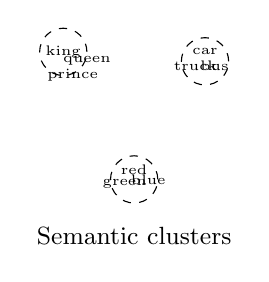
\begin{tikzpicture}[scale=0.6]
% Word clusters
\node[font=\tiny] at (-1.5,1.5) {king};
\node[font=\tiny] at (-1,1.3) {queen};
\node[font=\tiny] at (-1.3,1) {prince};

\node[font=\tiny] at (1.5,1.5) {car};
\node[font=\tiny] at (1.3,1.2) {truck};
\node[font=\tiny] at (1.7,1.2) {bus};

\node[font=\tiny] at (0,-1) {red};
\node[font=\tiny] at (0.3,-1.2) {blue};
\node[font=\tiny] at (-0.2,-1.3) {green};

\draw[dashed] (-1.5,1.5) circle (0.5);
\draw[dashed] (1.5,1.3) circle (0.5);
\draw[dashed] (0,-1.2) circle (0.5);

\node[below] at (0,-2) {\small Semantic clusters};
\end{tikzpicture}
\end{center}

\textbf{Special consideration:}\\
\small Cosine distance often better\\
than Euclidean for text
\end{columns}
\end{frame}

% SLIDE 40: Image Analysis
\begin{frame}
\frametitle{Application: Image Feature Analysis}
\begin{columns}[T]
\column{0.5\textwidth}
\textbf{Deep learning features:}
\begin{itemize}
\small
\item CNN embeddings
\item Last layer before classification
\item 512-2048 dimensions
\end{itemize}

\vspace{0.3cm}
\textbf{Use cases:}
\begin{itemize}
\small
\item Dataset exploration
\item Outlier detection
\item Class balance check
\item Model debugging
\end{itemize}

\vspace{0.3cm}
\textbf{Workflow:}\\
\small
Extract features → PCA → t-SNE

\column{0.5\textwidth}
\begin{center}
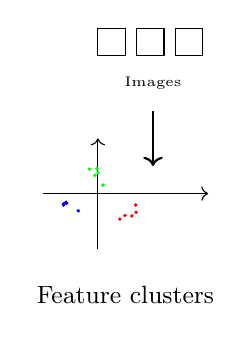
\begin{tikzpicture}[scale=0.7]
% Image patches to features
\draw (0,2) rectangle (0.5,2.5);
\draw (0.7,2) rectangle (1.2,2.5);
\draw (1.4,2) rectangle (1.9,2.5);
\node at (1,1.5) {\tiny Images};

\draw[->,thick] (1,1) -- (1,0);

% Feature space
\draw[->] (-1,-0.5) -- (2,-0.5);
\draw[->] (0,-1.5) -- (0,0.5);
\foreach \i in {1,...,5} {
    \fill[blue] ({-0.5+0.2*rand},{-0.8+0.2*rand}) circle (1pt);
    \fill[red] ({0.5+0.2*rand},{-0.8+0.2*rand}) circle (1pt);
    \fill[green] ({0+0.2*rand},{-0.2+0.2*rand}) circle (1pt);
}
\node[below] at (0.5,-2) {\small Feature clusters};
\end{tikzpicture}
\end{center}

\textbf{Note:} Similar images cluster\\
even without labels!
\end{columns}
\end{frame}

% SLIDE 41: Time-Series Applications
\begin{frame}
\frametitle{Application: Time-Series and Trajectories}
\begin{columns}[T]
\column{0.5\textwidth}
\textbf{Dynamic t-SNE:}
\begin{itemize}
\small
\item Sliding windows
\item Temporal regularization
\item Preserve trajectories
\end{itemize}

\vspace{0.3cm}
\textbf{Applications:}
\begin{itemize}
\small
\item Patient monitoring
\item Financial markets
\item System states
\item Behavior patterns
\end{itemize}

\vspace{0.3cm}
\textbf{Modified objective:}
$$C = KL(P||Q) + \lambda \sum_t \|\mathbf{Y}^t - \mathbf{Y}^{t-1}\|^2$$

\column{0.5\textwidth}
\begin{center}
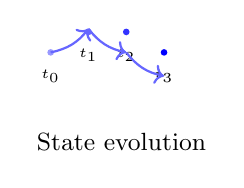
\begin{tikzpicture}[scale=0.6]
% Time evolution
\foreach \t in {0,1,2,3} {
    \pgfmathsetmacro{\x}{-1.5+\t*0.8}
    \pgfmathsetmacro{\y}{0.5*sin(\t*60)}
    \fill[blue!\the\numexpr40+\t*20\relax] (\x,\y) circle (2pt);
    \node[font=\tiny] at (\x,\y-0.5) {$t_\t$};
}
% Draw trajectory
\draw[->,thick,blue!60] (-1.5,0) to[bend right=20] (-0.7,0.5);
\draw[->,thick,blue!60] (-0.7,0.5) to[bend right=20] (0.1,0);
\draw[->,thick,blue!60] (0.1,0) to[bend right=20] (0.9,-0.5);

\node[below] at (0,-1.5) {\small State evolution};
\end{tikzpicture}
\end{center}

\textbf{Challenge:}\\
\small Balance stability vs. change
\end{columns}
\end{frame}

% SLIDE 42: Domain-Specific Tips
\begin{frame}
\frametitle{Domain-Specific Considerations}
\begin{columns}[T]
\column{0.5\textwidth}
\textbf{Biology:}
\begin{itemize}
\small
\item Handle sparsity
\item Log transform counts
\item Remove batch effects
\item Perplexity = 30-100
\end{itemize}

\vspace{0.2cm}
\textbf{Text:}
\begin{itemize}
\small
\item TF-IDF preprocessing
\item Cosine distance
\item Remove stop words
\item Perplexity = 5-50
\end{itemize}

\vspace{0.2cm}
\textbf{Images:}
\begin{itemize}
\small
\item Use pretrained features
\item Data augmentation aware
\item Perplexity = 30-50
\end{itemize}

\column{0.5\textwidth}
\textbf{Common pitfalls by domain:}

\begin{center}
\small
\begin{tabular}{|l|l|}
\hline
Domain & Pitfall \\
\hline
Biology & Batch effects \\
Text & Rare words \\
Images & Class imbalance \\
Finance & Temporal leakage \\
\hline
\end{tabular}
\end{center}

\vspace{0.3cm}
\textbf{Universal tip:}\\
\small Always validate with domain knowledge!

\vspace{0.3cm}
\textbf{Remember:}\\
\small t-SNE is exploratory, not definitive
\end{columns}
\end{frame}

% SLIDE 43: Gradient Derivation Part 1
\begin{frame}
\frametitle{Mathematical Deep Dive: Gradient Derivation (1/2)}
\begin{columns}[T]
\column{0.5\textwidth}
\textbf{Objective function:}
$$C = \sum_{ij} p_{ij} \log\frac{p_{ij}}{q_{ij}}$$

\textbf{Step 1: Derivative of $\log q_{ij}$}
$$q_{ij} = \frac{(1+d_{ij}^2)^{-1}}{Z}$$
where $Z = \sum_{k<l}(1+d_{kl}^2)^{-1}$

$$\frac{\partial \log q_{ij}}{\partial \mathbf{y}_i} = \frac{1}{q_{ij}}\frac{\partial q_{ij}}{\partial \mathbf{y}_i}$$

\column{0.5\textwidth}
\textbf{Step 2: Chain rule}
\small
$$\frac{\partial q_{ij}}{\partial \mathbf{y}_i} = \frac{\partial}{\partial \mathbf{y}_i}\left[\frac{(1+d_{ij}^2)^{-1}}{Z}\right]$$

Using quotient rule:
$$= \frac{-2(\mathbf{y}_i-\mathbf{y}_j)(1+d_{ij}^2)^{-2}Z + (1+d_{ij}^2)^{-1}\frac{\partial Z}{\partial \mathbf{y}_i}}{Z^2}$$
\end{columns}
\end{frame}

% SLIDE 44: Gradient Derivation Part 2  
\begin{frame}
\frametitle{Mathematical Deep Dive: Gradient Derivation (2/2)}
\begin{columns}[T]
\column{0.5\textwidth}
\textbf{Step 3: Simplify}

After algebra:
$$\frac{\partial C}{\partial \mathbf{y}_i} = 4\sum_j (p_{ij} - q_{ij})F_{ij}(\mathbf{y}_i - \mathbf{y}_j)$$

where $F_{ij} = (1 + d_{ij}^2)^{-1}$

\vspace{0.3cm}
\textbf{Interpretation:}
\begin{itemize}
\small
\item $(p_{ij} - q_{ij})$: error signal
\item $F_{ij}$: weight function  
\item $(\mathbf{y}_i - \mathbf{y}_j)$: direction
\end{itemize}

\column{0.5\textwidth}
\textbf{Beautiful symmetry:}

Force on point $i$ from $j$:
$$\mathbf{F}_{ij} = 4(p_{ij} - q_{ij})\frac{\mathbf{y}_i - \mathbf{y}_j}{1 + \|\mathbf{y}_i - \mathbf{y}_j\|^2}$$

\vspace{0.3cm}
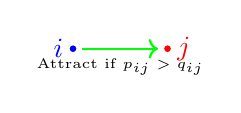
\begin{tikzpicture}[scale=0.6]
\fill[blue] (0,0) circle (2pt) node[left] {$i$};
\fill[red] (2,0) circle (2pt) node[right] {$j$};
\draw[->,thick,green] (0.2,0) -- (1.8,0);
\node[below] at (1,0) {\tiny Attract if $p_{ij} > q_{ij}$};
\end{tikzpicture}

\textbf{Note:} Student-t kernel appears\\
naturally in gradient!
\end{columns}
\end{frame}

% SLIDE 45: Initialization Strategies
\begin{frame}
\frametitle{Initialization Strategies}
\begin{columns}[T]
\column{0.5\textwidth}
\textbf{1. Random initialization:}
$$\mathbf{Y} \sim \mathcal{N}(0, \sigma^2 I)$$
\begin{itemize}
\small
\item Classic: $\sigma = 10^{-4}$
\item Spread out: $\sigma = 0.01$
\item Risk: poor local minima
\end{itemize}

\vspace{0.3cm}
\textbf{2. PCA initialization:}
$$\mathbf{Y} = [\mathbf{v}_1, \mathbf{v}_2]^T \mathbf{X}$$
\begin{itemize}
\small
\item First 2 principal components
\item Preserves global structure
\item Faster convergence
\end{itemize}

\column{0.5\textwidth}
\textbf{3. Spectral initialization:}

Graph Laplacian eigenvectors

\vspace{0.3cm}
\begin{center}
\begin{tikzpicture}[scale=0.5]
% Random init
\node at (0,2) {\tiny Random};
\foreach \i in {1,...,10} {
    \pgfmathsetmacro{\x}{rand}
    \pgfmathsetmacro{\y}{rand}
    \fill[gray] (\x,\y) circle (1pt);
}

% PCA init
\begin{scope}[shift={(4,0)}]
\node at (0,2) {\tiny PCA};
\foreach \i in {1,...,10} {
    \pgfmathsetmacro{\x}{0.8*rand}
    \pgfmathsetmacro{\y}{0.3*rand}
    \fill[gray] (\x,\y) circle (1pt);
}
\end{scope}
\end{tikzpicture}
\end{center}

\textbf{Impact on convergence:}\\
\small PCA: 500 iterations\\
Random: 1000 iterations
\end{columns}
\end{frame}

% SLIDE 46: Advanced Initialization
\begin{frame}
\frametitle{Advanced Initialization: Smart Strategies}
\begin{columns}[T]
\column{0.5\textwidth}
\textbf{Scaled PCA init:}
\begin{enumerate}
\small
\item Compute PCA
\item Scale to match t-dist variance
\item $\mathbf{Y} = \alpha [\mathbf{v}_1, \mathbf{v}_2]^T \mathbf{X}$
\item $\alpha = 0.0001 \times \max(|\mathbf{X}|)$
\end{enumerate}

\vspace{0.3cm}
\textbf{Why scaling matters:}\\
\small Initial $q_{ij}$ should be uniform\\
Prevents early clustering

\column{0.5\textwidth}
\textbf{Experimental results:}
\begin{center}
\small
\begin{tabular}{|l|c|c|}
\hline
Init & KL final & Time \\
\hline
Random & 1.82 & 45s \\
PCA & 1.65 & 30s \\
Scaled PCA & 1.58 & 25s \\
\hline
\end{tabular}
\end{center}

\vspace{0.3cm}
\textbf{Recommendation:}\\
\small Always use PCA initialization\\
unless specific reason not to
\end{columns}
\end{frame}

% SLIDE 47: Reading t-SNE Plots
\begin{frame}
\frametitle{How to Read t-SNE Plots}
\begin{columns}[T]
\column{0.5\textwidth}
\textbf{DO interpret:}
\begin{itemize}
\small
\item ✓ Clusters existence
\item ✓ Within-cluster structure  
\item ✓ Local neighborhoods
\item ✓ Relative density
\end{itemize}

\vspace{0.3cm}
\textbf{DON'T interpret:}
\begin{itemize}
\small
\item ✗ Cluster sizes
\item ✗ Between-cluster distances
\item ✗ Absolute positions
\item ✗ Empty space meaning
\end{itemize}

\column{0.5\textwidth}
\begin{center}
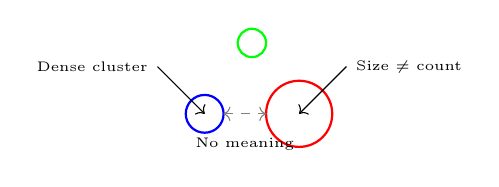
\begin{tikzpicture}[scale=0.6]
% Example plot with annotations
\draw[thick,blue] (0,0) circle (0.4);
\draw[thick,red] (2,0) circle (0.7);
\draw[thick,green] (1,1.5) circle (0.3);

\draw[<->,gray,dashed] (0.4,0) -- (1.3,0);
\node[below] at (0.85,-0.3) {\tiny No meaning};

\draw[<-] (0,0) -- (-1,1);
\node[left] at (-1,1) {\tiny Dense cluster};

\draw[<-] (2,0) -- (3,1);
\node[right] at (3,1) {\tiny Size $\neq$ count};
\end{tikzpicture}
\end{center}

\textbf{Golden rule:}\\
\small Confirm patterns with other methods
\end{columns}
\end{frame}

% SLIDE 48: Visual Artifacts
\begin{frame}
\frametitle{Common Visual Artifacts}
\begin{columns}[T]
\column{0.5\textwidth}
\textbf{1. Clumping:}
\begin{center}
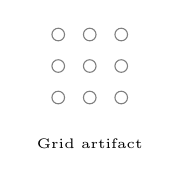
\begin{tikzpicture}[scale=0.4]
\foreach \i in {1,...,3} {
    \foreach \j in {1,...,3} {
        \draw[gray] (\i,\j) circle (0.2);
    }
}
\node[below] at (2,0) {\tiny Grid artifact};
\end{tikzpicture}
\end{center}
Cause: Optimization stuck

\vspace{0.2cm}
\textbf{2. Outlier chains:}
\begin{center}
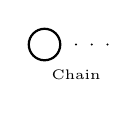
\begin{tikzpicture}[scale=0.4]
\draw[thick] (0,0) circle (0.5);
\fill (1,0) circle (1pt);
\fill (1.5,0) circle (1pt);
\fill (2,0) circle (1pt);
\node[below] at (1,-0.5) {\tiny Chain};
\end{tikzpicture}
\end{center}
Cause: Early stopping

\column{0.5\textwidth}
\textbf{3. Pinched clusters:}
\begin{center}
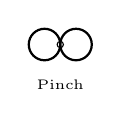
\begin{tikzpicture}[scale=0.4]
\draw[thick] (0,0) circle (0.5);
\draw[thick] (1,0) circle (0.5);
\draw (0.5,0) circle (0.1);
\node[below] at (0.5,-0.8) {\tiny Pinch};
\end{tikzpicture}
\end{center}
Cause: Perplexity too high

\vspace{0.2cm}
\textbf{Solutions:}
\begin{itemize}
\small
\item Run longer
\item Adjust perplexity
\item Check convergence
\item Multiple runs
\end{itemize}
\end{columns}
\end{frame}

% SLIDE 49: Statistical Validation
\begin{frame}
\frametitle{Statistical Validation of Clusters}
\begin{columns}[T]
\column{0.5\textwidth}
\textbf{Silhouette score:}
$$s_i = \frac{b_i - a_i}{\max(a_i, b_i)}$$
\begin{itemize}
\small
\item $a_i$: mean intra-cluster dist
\item $b_i$: mean nearest-cluster dist
\item Range: [-1, 1]
\end{itemize}

\vspace{0.3cm}
\textbf{Hopkins statistic:}\\
\small Tests clustering tendency\\
$H > 0.75$: clusterable

\column{0.5\textwidth}
\textbf{Permutation test:}
\begin{enumerate}
\small
\item Run t-SNE on real data
\item Measure cluster quality $Q$
\item Shuffle labels 100 times
\item Run t-SNE on shuffled
\item Compare $Q$ to null distribution
\end{enumerate}

\vspace{0.3cm}
\begin{center}
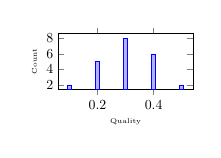
\begin{tikzpicture}[scale=0.5]
\begin{axis}[
    width=5cm, height=3cm,
    xlabel={\tiny Quality},
    ylabel={\tiny Count},
    ybar,
    bar width=3pt
]
\addplot coordinates {
    (0.1,2) (0.2,5) (0.3,8) (0.4,6) (0.5,2)
};
\draw[red,thick] (axis cs:0.7,0) -- (axis cs:0.7,10);
\node at (axis cs:0.7,11) {\tiny Real};
\end{axis}
\end{tikzpicture}
\end{center}
\end{columns}
\end{frame}

% SLIDE 50: Cross-validation
\begin{frame}
\frametitle{Cross-validation for t-SNE}
\begin{columns}[T]
\column{0.5\textwidth}
\textbf{Problem:}\\
\small Can't embed test points directly

\vspace{0.3cm}
\textbf{Solution 1: Parametric t-SNE}\\
\small Learn mapping function

\vspace{0.3cm}
\textbf{Solution 2: Out-of-sample}
\begin{enumerate}
\small
\item Run t-SNE on training
\item Fix training positions  
\item Optimize test positions only
\end{enumerate}

\column{0.5\textwidth}
\textbf{k-NN classification test:}
\begin{enumerate}
\small
\item Embed training data
\item Place test points
\item k-NN in 2D space
\item Measure accuracy
\end{enumerate}

\vspace{0.3cm}
\textbf{Results:}
\begin{center}
\small
\begin{tabular}{|l|c|}
\hline
Space & Accuracy \\
\hline
Original & 95\% \\
t-SNE 2D & 88\% \\
Random 2D & 45\% \\
\hline
\end{tabular}
\end{center}
\end{columns}
\end{frame}

% SLIDE 51: Troubleshooting Guide
\begin{frame}
\frametitle{Troubleshooting Guide}
\begin{columns}[T]
\column{0.5\textwidth}
\textbf{Problem: One big blob}
\begin{itemize}
\small
\item Increase perplexity
\item Run longer
\item Check data scale
\end{itemize}

\textbf{Problem: Too many clusters}
\begin{itemize}
\small
\item Decrease perplexity  
\item Check duplicates
\item PCA preprocessing
\end{itemize}

\textbf{Problem: Strange shapes}
\begin{itemize}
\small
\item Increase iterations
\item Check for outliers
\item Try different init
\end{itemize}

\column{0.5\textwidth}
\textbf{Diagnostic checklist:}
\begin{enumerate}
\small
\item KL decreasing? ✓
\item Gradient → 0? ✓
\item Multiple runs similar? ✓
\item Different perplexities? ✓
\item PCA looks reasonable? ✓
\end{enumerate}

\vspace{0.3cm}
\textbf{Emergency fixes:}
\begin{itemize}
\small
\item Subsample to debug
\item Remove outliers
\item Try UMAP instead
\end{itemize}
\end{columns}
\end{frame}

% SLIDE 52: Common Mistakes
\begin{frame}
\frametitle{Top 10 Common Mistakes}
\begin{columns}[T]
\column{0.5\textwidth}
\begin{enumerate}
\small
\item Not standardizing data
\item Single perplexity value
\item Too few iterations
\item Interpreting distances
\item Ignoring convergence
\item No PCA preprocessing
\item Wrong distance metric
\item Single random seed
\item Over-interpreting
\item Not validating
\end{enumerate}

\column{0.5\textwidth}
\textbf{How to avoid:}
\begin{itemize}
\small
\item Always standardize
\item Try 3+ perplexities
\item Min 1000 iterations
\item Focus on local structure
\item Check KL curve
\item PCA to 50D first
\item Match metric to data
\item Run 5+ times
\item Confirm with other methods
\item Use validation metrics
\end{itemize}
\end{columns}
\end{frame}

% SLIDE 53: Complete Pipeline Summary
\begin{frame}
\frametitle{The Complete t-SNE Pipeline}
\begin{center}
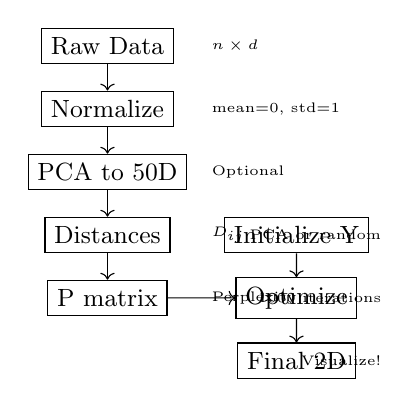
\begin{tikzpicture}[scale=0.8, node distance=1.5cm]
% Nodes
\node[draw, rectangle] (data) at (0,3) {\small Raw Data};
\node[draw, rectangle] (norm) at (0,2) {\small Normalize};
\node[draw, rectangle] (pca) at (0,1) {\small PCA to 50D};
\node[draw, rectangle] (dist) at (0,0) {\small Distances};
\node[draw, rectangle] (prob) at (0,-1) {\small P matrix};
\node[draw, rectangle] (init) at (3,0) {\small Initialize Y};
\node[draw, rectangle] (opt) at (3,-1) {\small Optimize};
\node[draw, rectangle] (embed) at (3,-2) {\small Final 2D};

% Arrows
\draw[->] (data) -- (norm);
\draw[->] (norm) -- (pca);
\draw[->] (pca) -- (dist);
\draw[->] (dist) -- (prob);
\draw[->] (prob) -- (opt);
\draw[->] (init) -- (opt);
\draw[->] (opt) -- (embed);

% Annotations
\node[right] at (1.5,3) {\tiny $n \times d$};
\node[right] at (1.5,2) {\tiny mean=0, std=1};
\node[right] at (1.5,1) {\tiny Optional};
\node[right] at (1.5,0) {\tiny $D_{ij}$};
\node[right] at (1.5,-1) {\tiny Perplexity};
\node[left] at (4.5,0) {\tiny PCA or random};
\node[left] at (4.5,-1) {\tiny 1000 iterations};
\node[left] at (4.5,-2) {\tiny Visualize!};
\end{tikzpicture}
\end{center}
\end{frame}

% SLIDE 54: Mathematical Synthesis
\begin{frame}
\frametitle{Mathematical Journey: Synthesis}
\begin{columns}[T]
\column{0.5\textwidth}
\textbf{From distances to geometry:}
\begin{enumerate}
\small
\item Distances: $D_{ij} = \|\mathbf{x}_i - \mathbf{x}_j\|$
\item Similarities: $s_{ij} = e^{-D_{ij}^2/2\sigma_i^2}$
\item Probabilities: $p_{ij} = s_{ij}/\sum_{kl} s_{kl}$
\item Embedding: $\min_Y KL(P||Q)$
\item Forces: $\nabla = 4(P-Q) \odot F \odot D$
\end{enumerate}

\vspace{0.3cm}
\textbf{Key insights:}
\begin{itemize}
\small
\item Local $>$ global
\item Relative $>$ absolute
\item Adaptive $>$ fixed
\end{itemize}

\column{0.5\textwidth}
\textbf{The mathematics that matters:}
\begin{itemize}
\small
\item \textbf{Information:} KL divergence
\item \textbf{Probability:} Conditional → Joint
\item \textbf{Optimization:} Non-convex
\item \textbf{Geometry:} Manifold learning
\item \textbf{Statistics:} Heavy tails
\end{itemize}

\vspace{0.3cm}
\textbf{Unified view:}\\
\small t-SNE = Information geometry\\
+ Stochastic neighbors\\
+ Heavy-tailed embeddings
\end{columns}
\end{frame}

% SLIDE 55: The Recipe
\begin{frame}
\frametitle{The t-SNE Recipe: Your Go-To Guide}
\begin{columns}[T]
\column{0.5\textwidth}
\textbf{Ingredients:}
\begin{itemize}
\small
\item Data matrix: $n \times d$
\item Perplexity: 30 (default)
\item Iterations: 1000
\item Learning rate: 200 or $n/12$
\end{itemize}

\vspace{0.3cm}
\textbf{Instructions:}
\begin{enumerate}
\small
\item Center \& scale data
\item PCA to 50D (if $d > 50$)
\item Set perplexity $\in [5, 50]$
\item Initialize with PCA
\item Run with early exaggeration
\item Check convergence
\item Try 3 perplexities
\item Run 5 times
\end{enumerate}

\column{0.5\textwidth}
\textbf{Quality control:}
\begin{itemize}
\small
\item ✓ KL decreasing?
\item ✓ Clusters stable?
\item ✓ Known structure visible?
\item ✓ No artifacts?
\end{itemize}

\vspace{0.3cm}
\textbf{Serving suggestions:}
\begin{itemize}
\small
\item Color by known labels
\item Interactive plot (plotly)
\item Compare with PCA
\item Validate with clustering
\end{itemize}

\vspace{0.3cm}
\textbf{Warning:}\\
\small Never trust distances!\\
Always run multiple times!
\end{columns}
\end{frame}

% SLIDE 56: Future Research
\begin{frame}
\frametitle{Open Problems and Future Directions}
\begin{columns}[T]
\column{0.5\textwidth}
\textbf{Theoretical challenges:}
\begin{enumerate}
\small
\item Convergence guarantees
\item Optimal perplexity theory
\item Embedding quality bounds
\item Statistical consistency
\item Manifold reconstruction
\end{enumerate}

\vspace{0.3cm}
\textbf{Algorithmic advances:}
\begin{enumerate}
\small
\item Linear time algorithms
\item Online/streaming t-SNE
\item Automatic hyperparameters
\item Interpretable embeddings
\end{enumerate}

\column{0.5\textwidth}
\textbf{Applications frontier:}
\begin{itemize}
\small
\item Million-point datasets
\item Real-time visualization
\item 3D and VR embedding
\item Temporal dynamics
\item Multi-modal data
\end{itemize}

\vspace{0.3cm}
\textbf{Your contribution?}\\
\small Many problems remain open!\\
Combine theory + practice
\end{columns}
\end{frame}

% SLIDE 57: Deep Learning Connection
\begin{frame}
\frametitle{t-SNE in the Deep Learning Era}
\begin{columns}[T]
\column{0.5\textwidth}
\textbf{Visualizing deep networks:}
\begin{itemize}
\small
\item Layer activations
\item Learned representations
\item Attention patterns
\item Embedding spaces
\end{itemize}

\vspace{0.3cm}
\textbf{Model debugging:}
\begin{itemize}
\small
\item Feature collapse
\item Class separation
\item Adversarial examples
\item Transfer learning
\end{itemize}

\column{0.5\textwidth}
\begin{center}
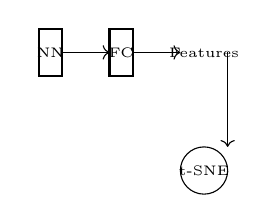
\begin{tikzpicture}[scale=0.6]
% Neural network to t-SNE
\draw[thick] (0,1) rectangle (0.5,2);
\node at (0.25,1.5) {\tiny NN};
\draw[->] (0.5,1.5) -- (1.5,1.5);
\draw[thick] (1.5,1) rectangle (2,2);
\node at (1.75,1.5) {\tiny FC};
\draw[->] (2,1.5) -- (3,1.5);
\node at (3.5,1.5) {\tiny Features};
\draw[->] (4,1.5) -- (4,-0.5);
\draw (3.5,-1) circle (0.5);
\node at (3.5,-1) {\tiny t-SNE};
\end{tikzpicture}
\end{center}

\textbf{Integration approaches:}
\begin{enumerate}
\small
\item Extract → t-SNE → Visualize
\item Joint training (parametric)
\item Regularization with t-SNE
\end{enumerate}
\end{columns}
\end{frame}

% SLIDE 58: Complete Example
\begin{frame}
\frametitle{Complete Example: Iris Dataset}
\begin{columns}[T]
\column{0.5\textwidth}
\textbf{Data:}
\begin{itemize}
\small
\item 150 samples, 4 features
\item 3 species (50 each)
\item Classic test case
\end{itemize}

\textbf{Steps:}
\begin{enumerate}
\footnotesize
\item Load: $(150 \times 4)$ matrix
\item Scale: mean=0, std=1
\item Distances: Euclidean
\item Perplexity: 30
\item $\sigma$ search: $[0.1, 10]$
\item P matrix: symmetrize
\item Init: PCA × 0.0001
\item Optimize: 1000 iterations
\end{enumerate}

\column{0.5\textwidth}
\textbf{Results:}
\begin{center}
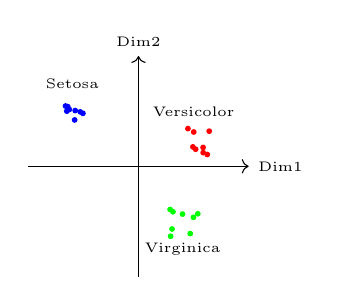
\begin{tikzpicture}[scale=0.7]
\draw[->] (-2,0) -- (2,0) node[right] {\tiny Dim1};
\draw[->] (0,-2) -- (0,2) node[above] {\tiny Dim2};
% Setosa
\foreach \i in {1,...,8} {
    \pgfmathsetmacro{\x}{-1.2+0.2*rand}
    \pgfmathsetmacro{\y}{1+0.2*rand}
    \fill[blue] (\x,\y) circle (1.5pt);
}
% Versicolor  
\foreach \i in {1,...,8} {
    \pgfmathsetmacro{\x}{1+0.3*rand}
    \pgfmathsetmacro{\y}{0.5+0.3*rand}
    \fill[red] (\x,\y) circle (1.5pt);
}
% Virginica
\foreach \i in {1,...,8} {
    \pgfmathsetmacro{\x}{0.8+0.3*rand}
    \pgfmathsetmacro{\y}{-1+0.3*rand}
    \fill[green] (\x,\y) circle (1.5pt);
}
\node at (-1.2,1.5) {\tiny Setosa};
\node at (1,1) {\tiny Versicolor};
\node at (0.8,-1.5) {\tiny Virginica};
\end{tikzpicture}
\end{center}

Perfect separation achieved!
\end{columns}
\end{frame}

% SLIDE 59: Key Takeaways
\begin{frame}
\frametitle{Key Takeaways: What to Remember}
\begin{columns}[T]
\column{0.5\textwidth}
\textbf{Core concepts:}
\begin{enumerate}
\small
\item Preserves neighborhoods, not distances
\item Probabilities > distances
\item Heavy tails solve crowding
\item Non-convex optimization
\item Multiple runs essential
\end{enumerate}

\vspace{0.3cm}
\textbf{Practical wisdom:}
\begin{itemize}
\small
\item Always standardize
\item Try multiple perplexities
\item PCA preprocessing helps
\item Validate findings
\end{itemize}

\column{0.5\textwidth}
\textbf{Mathematical insights:}
\begin{itemize}
\small
\item KL divergence for matching
\item Student-t for heavy tails
\item Gradient = attractive/repulsive forces
\item Adaptive bandwidth crucial
\end{itemize}

\vspace{0.3cm}
\textbf{Remember:}\\
\small t-SNE is a tool for exploration,\\
not proof!\\
\vspace{0.3cm}
Use wisely, interpret carefully
\end{columns}
\end{frame}

% SLIDE 60: Closing
\begin{frame}
\frametitle{Final Thoughts: The Art and Science of t-SNE}
\begin{center}
\vspace{0.5cm}
{\large t-SNE bridges mathematics and intuition}

\vspace{0.5cm}
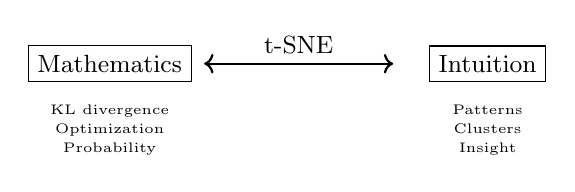
\begin{tikzpicture}[scale=0.8]
% Mathematical foundation
\node[draw, rectangle] at (-3,0) {\small Mathematics};
\node[below] at (-3,-0.5) {\tiny KL divergence};
\node[below] at (-3,-0.8) {\tiny Optimization};
\node[below] at (-3,-1.1) {\tiny Probability};

% Bridge
\draw[thick, <->] (-1.5,0) -- (1.5,0);
\node[above] at (0,0) {\small t-SNE};

% Visual understanding  
\node[draw, rectangle] at (3,0) {\small Intuition};
\node[below] at (3,-0.5) {\tiny Patterns};
\node[below] at (3,-0.8) {\tiny Clusters};
\node[below] at (3,-1.1) {\tiny Insight};
\end{tikzpicture}

\vspace{0.5cm}
\textbf{You now have:}
\begin{itemize}
\item Mathematical understanding
\item Practical skills
\item Critical perspective
\end{itemize}

\vspace{0.5cm}
{\large \textit{Go forth and visualize responsibly!}}
\end{center}
\end{frame}

\end{document}